%!TEX root = presentazionelancia.tex

\setlength{\parskip}{\baselineskip} 
\section{Primeros pasos}
\begin{frame}[t]
\frametitle{\insertsection}
\begin{block}{¿Qué es \LaTeX{} \& friends?}
	Es un taller tiene como metas
	\begin{itemize}
		\item duración hasta fin de ciclo.
	 	\item resolución de los ejercicios de los libros
	 	\item embeber y extender \TeX{} a Python, plataformas web (MathJax, Ka\TeX, MathML) y plataformas de escritorio.
	 	\item presentar informes matemáticos de alta calidad.
	 \end{itemize} 
\end{block}
\end{frame}

%\begin{frame}
%\frametitle{The social graph}
%Facebook has more than 1 billion active user 
%\begin{itemize}
%	\item recording relationships,
%	\item sharing interests,
%	\item uploading pictures and \dots
%\end{itemize}
%
%The user experience of Fb comes from rapid, efficient and scalable access to the \emph{social graph}
%\end{frame}
%
%\begin{frame}
%	What's behind an entry in yours Fb page?
%
%	A single Fb page aggregate and filter hundreds of items from the social graph.
%\end{frame}%

%\begin{frame}[t]
%\begin{center}
%\includegraphics[width=\paperheight]{figs/gitter}	
%\end{center}


%\end{frame}
%%%
{
	\usebackgroundtemplate{\centering\includegraphics[width=\paperwidth]{gitter}}
	\begin{frame}[plain]
\end{frame}
}
%%%%
%\begin{frame}
%\frametitle{Before Tao}
%	\begin{itemize}
% 	\item Facebook was storing the social graph to MySql
%	\begin{itemize}
%		\item  	Quering it from PHP
%		\item  	Storing result in memcache\\
%	\end{itemize}
%	\end{itemize}
%	\begin{center}
%		\includegraphics[width=0.3\textwidth]{figs/php-logo.eps}\quad
%		\includegraphics[width=0.3\textwidth]{figs/mysql.png}
%	\end{center}
% 	Over time Fb deprecated direct access to MySQL in favor of a graph (associations, nodes) abstraction
%\end{frame}

%\begin{frame}
%\frametitle{Limits}
%    \begin{itemize}
%    	\item Operations on lists are inefficient in memcache (update whole list)
%    	\item Complexity on clients managing cache
%    	\item Hard to offer read-after-write consistency
%    \end{itemize}
%Also they want to access social graph from non-PHP services
%\end{frame}
%
%\begin{frame}
%\frametitle{TAO's Goals}
%	\begin{itemize}
%		\item Efficiency at Scale
%		\pause
%		\item Low read latency
%		\pause
%		\item Timeliness of writes
%		\pause
%		\item High read availability
%	\end{itemize}
%\end{frame}
